\chapter{Introdução}

O ser humano vem usando a sua habilidade de reconhecimento de padrões desde  muito antes do início do processo civilizatório. Grupos de humanos paleolíticos já faziam registro dos padrões migratórios de certos grupos de cervídeos. Durante a aurora da revolução neolítica, nossa capacidade de reconhecimento de padrões foi direcionada para a agricultura com a criação de monumentos que registraram a mudança das estações ao longo do ano.

O cérebro humano evoluiu espantosamente. E no que se refere a quantidade de informação processada, o cérebro possui enorme vantagem em relação a quantidade de informação processada por um computador \citep{Hall2014}. Este não para de funcionar somente porque algumas células morrem. Um computador, por sua vez, não funciona quando há degradação da sua unidade central de processamento \citep{Mao1996}.

O campo do aprendizado de máquina aborda a criação de programas computacionais que automaticamente melhorem a si mesmos através da experiência \citep{Levy1997,Michie1994}. Tanto a rede neuronal quanto a árvore de decisão despontam como estratégias de solução para a resolução de problemas de reconhecimento de padrões \citep{MacKay2005}.


Uma rede neuronal artificial possui semelhanças com a rede neuronal natural, nesta o cômputo do cérebro é feito através de uma vasta quantidade de neurônios interconectados \citep{Feldman1988,Poulton2002}. A comunicação entre essas células é realizada através de impulsos elétricos. Tais impulsos elétricos são transmitidos e recebidos por meio de sinapses nervosas entre axônios e dendritos. As sinapses são estruturas elementares e uma unidade funcional localizada entre dois neurônios \citep{Krogh2008}. 

As Redes Neurais Artificiais são inspiradas em modelos sensoriais de processamento de tarefas realizadas pelo cérebro \citep{Hagan1996}. Uma RNA\footnote{RNA: Rede Neural Artificial}, portanto, pode ser criada através da aplicação de algoritmos matemáticos que imitem a tarefa realizada por um neurônio \citep{Nedjah2016}. 

Já a árvore de decisão auxilia na predição da classe de um objeto em um estudo com base em um treinamento prévio. Ou seja, funciona como um algoritmo de aprendizado de máquina supervisionado que é basicamente aplicado em problemas de classificação \citep{FreundYoav1999}. Funciona tanto para variáveis categóricas quando para variáveis dependentes. Nesse algoritmo, a população original é dividida em dois ou mais grupos de populações homogêneas \citep{Simard2000}. 

\section{Redes Neuronais Artificiais}

\citet{McCulloch1943} redigem o trabalho pioneiro onde foi modelado um neurônio cuja resposta dependia do \textit{input}\footnote{Valor de entrada} que provinha de outros neurônios e do peso utilizado.  Já \citet{Rosenblatt1962} cria a teoria de convergência do \textit{Perceptron} onde ele prova que modelos de neurônios possuem propriedades similares ao cérebro humano \citep{Kanal2001}. Neste sentido as redes neurais artificiais podem realizar performasses sofisticadas no reconhecimento de padrões, mesmo se alguns neurônios forem destruídos \citep{Levy1997}. \citet{Minsky1969} demonstraram que \textit{Perceptrons} somente resolvem uma classe muito limitada de problemas que podem ser linearizados.

Os primeiros artigos sobre redes neurais em geofísica datam de $1989$ e são focalizados basicamente em o que a RNA pode fazer com dados de natureza diferente. E como preparar o dado para inserir na rede para depois interpretá-lo. As redes neurais artificiais foram usualmente treinadas com dados sintéticos e depois testados em dados reais. Contudo, hoje é comum usar dados reais para treinar a rede \citep{Adibifard2014}. Embora, ambas as abordagens sejam aceitas. O foco a partir de $1995$ até o presente relaciona-se a algumas aplicações específicas, tais como caracterização de reservatórios. E a ênfase tem sido dada mais na integração de dados associado a uma interpretação compreensiva, ao contrário de uma aplicação isolada \citep{Poulton2002}. 

No problema específicos de poços, um passo importante é a identificação de topo e base de camadas que podem ser associadas com mudanças das propriedades petrofísicas \citep{Saljooghi2014}. Algoritmos baseados em derivadas nas curvas de log não identificam camadas muito finas, ou ruído \citep{Zhang1999}. \citet{Chakravarthy1999} consegue através do uso da função radial localizar os limites de camadas em alta definição em dados de log de indução (HDIL). Já \citet{Benaouda1999} consegue classificar tipos litológicos em poços parcialmente desmoronados através do uso da rede neuronal com propagação de erro e mudanças de classes a medida que prossegue a análise.

O neurônio de \citet{McCulloch1943} propõe um limite binário para a criação de um modelo. Este neurônio artificial registra uma soma de pesos de $n$ sinais de entrada, $x_{j}$, $j=1,2,3,...,n$, e fornece um \textit{output}\footnote{Valor de saída} de $1$ caso esta soma esteja acima do limite $u$. Caso contrário o \textit{output} é $0$. Matematicamente essa relação pode ser descrita de acordo com a Eq. \ref{Eq.neuronio-McCulloch}:

\begin{eqnarray}
y=\theta \left( \sum^{n}_{j=1} w_{j} x_{j} -u \right)
\label{Eq.neuronio-McCulloch}
\end{eqnarray}

Onde $\theta$ é o passo dado na posição $0$, $w_{j}$ é chamada sinapse-peso associado a um $j_{esimo}$ \textit{input}. A título de simplificação a função limite\footnote{Genericamente chamada de função de ativação} $u$ é considerada um outro peso $w_{0}=-u$ anexado a um neurônio com um \textit{input} constante $x_{0}=1$. Pesos positivos correspondem a uma sinapse \textbf{excitatória}, enquanto pesos negativos correspondem a uma sinapse \textbf{inibitória}. Este modelo contém uma série de simplificações que não refletem o verdadeiro comportamento dos neurônios biológicos \citep{Mao1996}.  

Derivações do neurônio de \citet{McCulloch1943} na escolha das funções de ativação. Uma função largamente utilizada é a função sigmóide, que exibe uma suavização dos \textit{outputs} a medida que o valor da função diminui \citep{Mao1996,Misra2010}. Essa função de ativação pode ser expressa de acordo com a Eq. \ref{f.sigmoide}:

\begin{eqnarray}
g(x)=1/(1+e^{-\beta x})
\label{f.sigmoide}
\end{eqnarray}

Onde $\beta$ é o parâmetro de inclinação. A Fig. \ref{Esquematico de McCulloch} ilustra a sequência lógica da operação de uma RNA para um neurônio simples de McCulloch-Pitts. 
\\
\begin{figure}[H]
	\centering
	\setlength{\fboxsep}{8pt}
	\setlength{\fboxrule}{0.1pt}
	\fbox{
	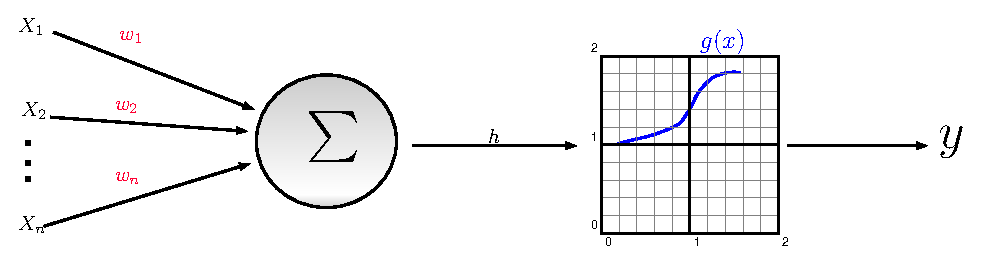
\includegraphics[scale=0.7]{Imagens/McCulloch.eps}
	}
	\caption{Modelo esquemático de um neurônio de McCulloch-Pitts. Onde $x_{1}, x_{2}, ..., x_{n}$ são os \textit{inputs}, $w_{1}, w_{2}, ..., w_{n}$ são os pesos, h é o treino, $g(x)$ é a função de ativação, e $y$ é o \textit{output}.}
	\label{Esquematico de McCulloch}
\end{figure}

Mais de $50$ tipos de redes neurais artificiais tem sido criadas até o ano de $2014$ \citep{Saljooghi2014}.

\section{Redes com aprendizado não-supervisionado}

Nesta categoria de RNA's são apenas inseridos os valores de atributos de entrada. Os valores de saída são definidos pela própria rede que passa por um processo de treinamento não supervionado. As redes que são submetidas a este tipo de treinamento são mais indicadas para tarefas aonde são exigidos agrupamento de dados (\textit{Clustering}). Neste processo uma classe deve ser atribuída aos registros da rede observando-se apenas o comportamento de seus atributos, no caso em particular deste trabalho tratam-se de propriedades geofísicas.

Uma rede com treinamento não supervisionado inspira-se no funcionamento do córtex cerebral. Neste modelo biológico, o organismo aprende a realizar alguma tarefa, por meio da identificação de padrões. Por exemplo, ao identificar uma música determinados padrões sonoros que compõe o conjunto harmonioso de notas precisam ser aprendidos antes de serem reconhecidos. Durante este processo, regiões específicas do cérebro vão sendo paulatinamente acionadas. Isto somente é possível, devido conexões específicas que são formadas entre os neurônios
presentes no córtex, Fig. \ref{homunculo}.

Os detalhes dos processos que regulam o córtex ainda não foram totalmente elucidados, contudo é seguro assumir que a primeira representação dos fenômenos que aprendemos, no mundo, pode ser representado por uma superfície topológica.  

\begin{figure}[H]
	\centering
	\setlength{\fboxsep}{8pt}
	\setlength{\fboxrule}{0.1pt}
	\fbox{
		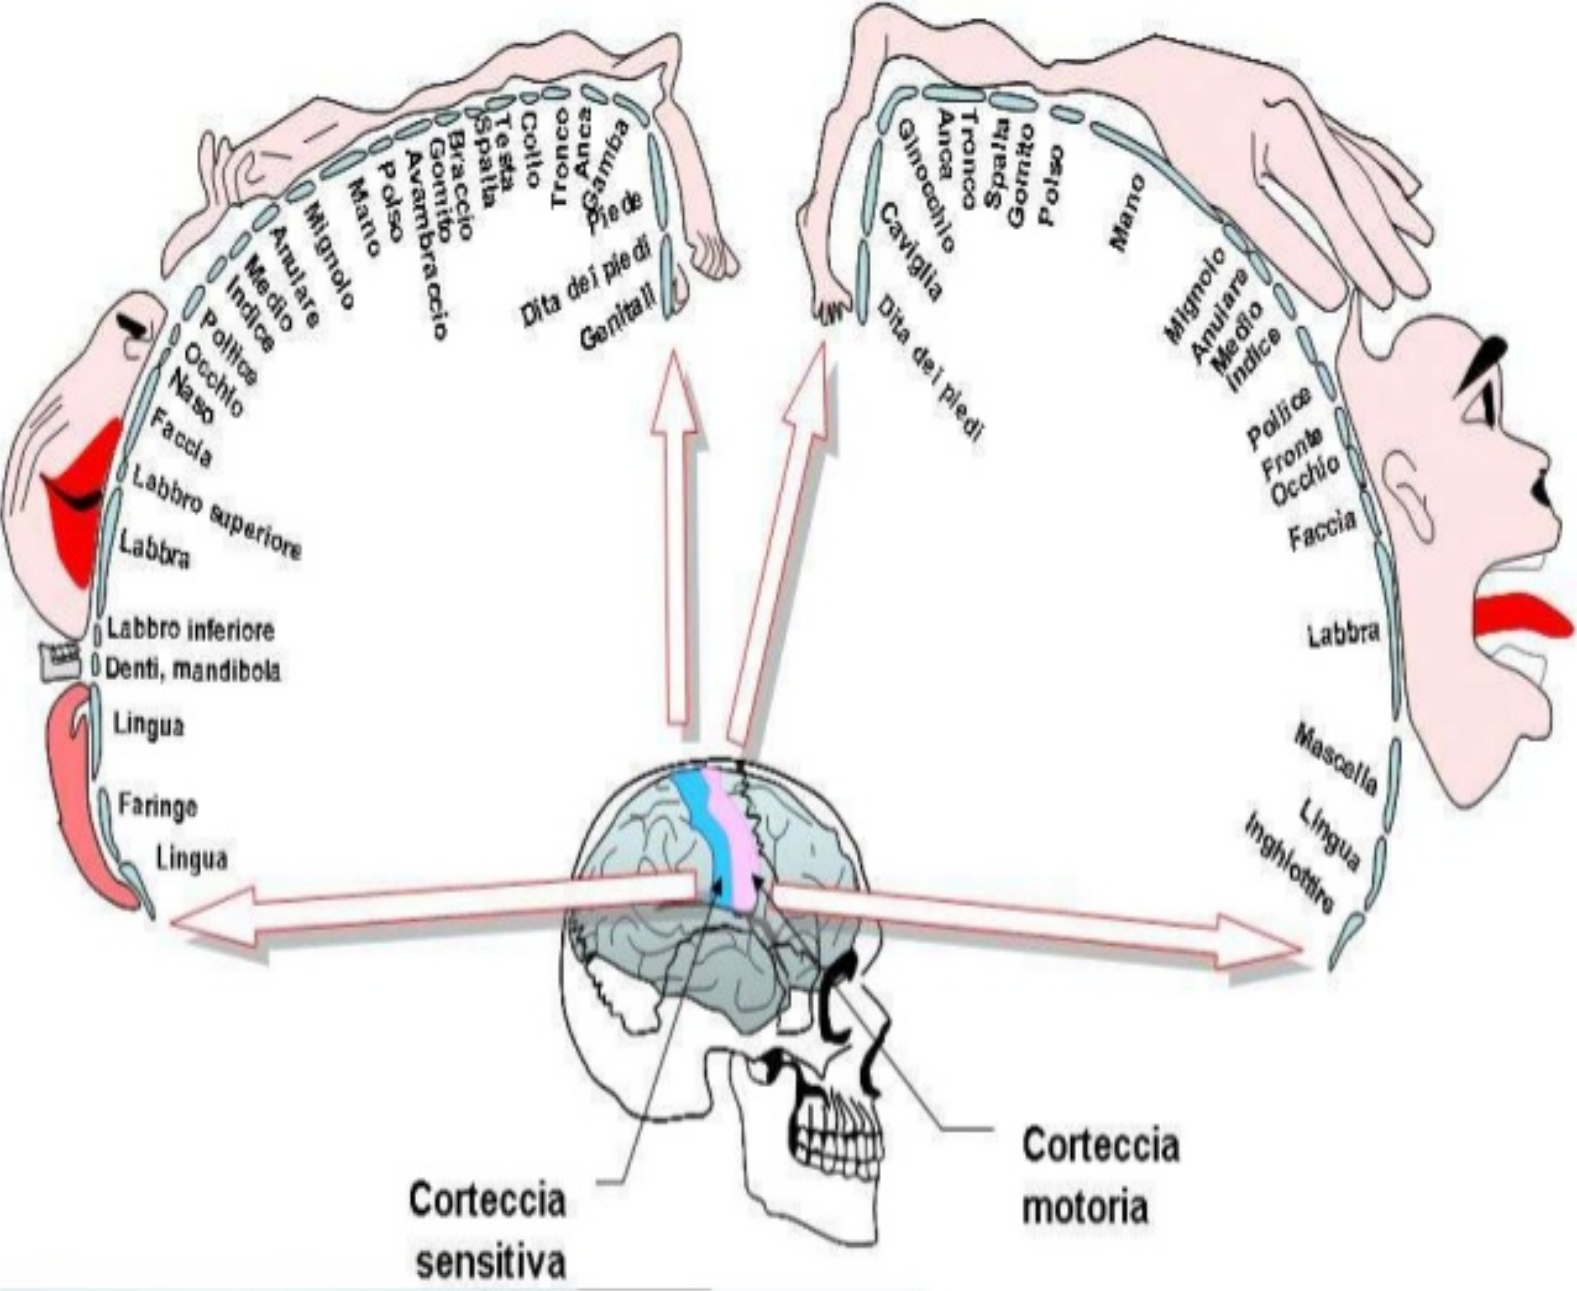
\includegraphics[scale=0.5]{Imagens/homunculo.png}
	}
	\caption{Homúnculo de Penfield.}
	\label{homunculo}
\end{figure}

Um cérebro que sofreu uma comossão grave perde a capacidade de acessar
determinadas zonas do homúnulo responsáveis por atividades específicas. Contudo
o cérebro tem a capacidade de destinar outras regiões para o controle destas
ações que foram previamente perdidas.

Além de casos graves como um acidente o cérebro também perde a capacidade de
aprendizado com o tempo. Em humanos, a capacidade de aprendizado vai da pequena
infância até a puberdade. Após este período, o cérebro passar a reter o que fora
aprendido. Sendo assim o aprendizado é uma função que depende, entre outras
coisas, do tempo.

\subsection{A Rede de Kohonen}

A localização espacial de um neurônio da saída em um mapa topográfico
corresponde a um domínio ou característica particular do dado retirado do espaço
de entrada. E estas entradas são mapeadas de forma ordenada, a exemplo dos mapas
cito-arqueturais do córtex cerebral.

Neste processo de identificação de padrões a redundância torna-se impreterível,
pois o neurônio da camada de saída que apresentar a maior resposta terá os seus
pesos ajustados. Além disso, o peso dos neurônios vizinhos também serão
ajustados em menor intensidade ao comparados com o neurônio vencedor.

Isto implica que os neurônios devem estar posicionados em um arranjo geométrico
adequado. Esta teoria é baseada na suposição de que as células nervosas
corticais estão organizadas anatomicamente em relação aos estímulos que recebem
dos sensores aos quais estão ligadas \citep{Artero2009}.

Este modelo exige a definição de vizinhança entre neurônios de forma geométrica.
Alguns arranjos são comumente utilizados, como por exemplo, os arranjos
triangulares, hexagonal, retangulares, etc.

No caso de arranjos retangulares, diferentes vizinhanças de um neurônio
$N_{i,j}$ podem ser configuradas em quartetos, diagonais e octetos. 

A Fig. \ref{hiperplano} ilustra o arranjo retangular e as vizinhanças, em quartetos, adotado neste trabalho. 

\begin{figure}[H]
	\centering
	\setlength{\fboxsep}{8pt}
	\setlength{\fboxrule}{0.1pt}
	\fbox{
		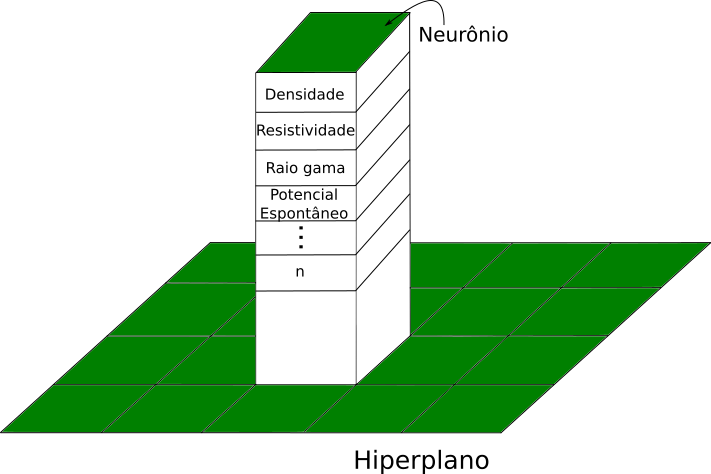
\includegraphics[scale=0.5]{Imagens/hiperplano.png}
	}
	\caption{Neurônio e suas vizinhanças}
	\label{hiperplano}
\end{figure}

O conceito de vizinhança representa uma competição pelo melhor aprendizado e o ajuste do vencedor e da sua vizinhança é um estímulo para que os neurônios ao redor do vencedor também melhorem.

Durante a etapa de treinamento é identificado o neurônio que tem os parâmetros de entrada mais parecidos com os valores dos pesos. Este procedimento é realizado via cálculo da distância euclidiana, Eq. \ref{euclidiana}, entre o parâmetro de entrada $x(t)$ e o peso $w_{i,j}$.

\begin{eqnarray}
d(t)= \sum^{n}_{i=1}[x(t)-w_{i,j}(t)]^{2}
\label{euclidiana}
\end{eqnarray}

